\documentclass[../practica.root.tex]{subfiles}

\begin{document}
\begin{enumerate}
    \item Dado $A = \{1, 2, 3\}$, indicar V ó F:
          \begin{enumerate}
              \item $1 \in A$ \cmark
              \item $\{1\} \subseteq A$ \cmark
              \item $\{2, 1\} \subseteq A$ \cmark
              \item $\{1, 3\} \in A$ \xmark
              \item $\{2\} \in A$ \xmark
          \end{enumerate}

    \item Dado $A = \{1, 2, \{3\}, \{1, 2\}\}$, indicar V ó F
          \begin{enumerate}
              \item $3 \in A$ \xmark
              \item $\{3\} \subseteq A$ \xmark
              \item $\{3\} \in A$ \cmark
              \item $\{\{3\}\} \subseteq A$ \cmark
              \item $\{1, 2\} \in A$ \cmark
              \item $\{1, 2\} \subseteq A$ \cmark
              \item $\{\{1, 2\}\} \subseteq A$ \cmark
              \item $\{\{1, 2\}, 3\} \subseteq A$ \xmark
              \item $\emptyset \in A$ \xmark
              \item $\emptyset \subseteq A$ \cmark
              \item $A \in A$ \xmark
              \item $A \subseteq A$ \cmark
          \end{enumerate}

    \item Determinar si $A \subseteq B$
          \begin{enumerate}
              \item $A = \{1, 2, 3\}$, $B = \{5, 4, 3, 2, 1\}$ \cmark
              \item $A = \{1, 2, 3\}$, $B = \{1, 2, \{3\}, -3\}$ \xmark
              \item $A = \{x \in \R / 2 < |x| < 3\}$, $B = \{x \in \R / x^2 < 3\}$ \xmark
              \item $A = \{\emptyset\}$, $B = \emptyset$ \xmark
          \end{enumerate}

    \item Describir por comprensión usando \textit{solo una} ecuación
          \begin{enumerate}
              \item
                    \[ \{-3, 1, 5\} = \{x \in \N / (x+3)(x-1)(x-5) = 0\} \]
                    \[ (-\infty, 2]\cup[7, +\infty) = \{x \in \R / (x-2)(x-7) \geq 0\}\]
              \item
                    \begin{enumerate}
                        \item $\{(x; y) \in \R^2 / x = y\}$
                        \item $\{(x; y) \in \R^2 / y-x = 0\}$
                        \item $\{(x; y) \in \R^2 / (y-x)(y+x) = 0\}$
                        \item $\{(x; y) \in \R^2 / (x-1)(x-2) = 0\}$
                        \item $\{(x; y) \in \R^2 / x = -1\}$
                        \item $\{(x; y) \in \R^2 / y < 0\}$
                    \end{enumerate}
          \end{enumerate}

    \item Dados $A = \{1, -2, 7, 3\}$, $B = \{1, \{3\}, 10\}$ y $C = \{-2, \{1, 2, 3\}, 3\}$, y
          $U = \{1, \{3\}, -2, 7, 10, \{1,2,3\},3\}$, hallar
          \begin{enumerate}
              \item $A \cap (B \triangle C)$
                    \[ B \triangle C = \{1, \{3\}, 10, -2 , \{1, 2, 3\}, 3\} \]
                    \begin{align*}
                        A \cap (B \triangle C) & = \{1, -2, 7, 3\}\cap\{1, \{3\}, 10, -2 , \{1, 2, 3\}, 3\} \\
                                               & = \boxed{\{1, -2, 3\}}
                    \end{align*}

              \item $(A \cap B)\triangle(A \cap C)$
                    \begin{align*}
                        A \cap B & =  \{1, -2, 7, 3\} \cap \{1, \{3\}, 10\} = \{1\}         \\
                        A \cap C & = \{1, -2, 7, 3\} \cap \{-2, \{1, 2, 3\}, 3\} = \{-2,3\}
                    \end{align*}
                    \[ \{1\} \triangle \{-2,3\} = \boxed{\{1, -2, 3\}}\]

              \item $A^c \cap B^c \cap C^c$
                    \begin{align*}
                        A^c & = \{\{3\}, 10, \{1, 2, 3\}\} \\
                        B^c & = \{-2, 7, \{1, 2, 3\}, 3\}  \\
                        C^c & = \{1, \{3\}, 7, 10\}
                    \end{align*}
                    \[ \{\{3\}, 10, \{1, 2, 3\}\} \cap \{-2, 7, \{1, 2, 3\}, 3\} \cap \{1, \{3\}, 7, 10\} \]
                    \[ \{ \{1, 2, 3\} \} \cap \{1, \{3\}, 7, 10\} = \boxed{\emptyset} \]
          \end{enumerate}

    \item Dados $A, B, C \subseteq V$, describir:
          \begin{enumerate}
              \item $(A \cup B \cup C)^c$ como intersecciones y complementos
                    \[ \boxed{A^c \cap B^c \cap C^c} \]
              \item $(A \cap B \cap C)^c$ como uniones y complementos
                    \[ \boxed{A^c \cup B^c \cup C^c} \]
          \end{enumerate}

    \item Representar en un diagrama de Venn: \\
          \begin{enumerate}
              \item $(A \cup B^c) \cap C$
              \item $A \triangle (B \cup C)$
              \item $(A \cup (B \triangle C)$
          \end{enumerate}
          \begin{figure}[h]
              \centering
              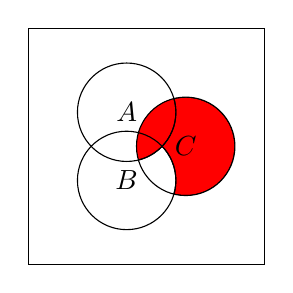
\begin{tikzpicture}[scale=0.5]
                  \draw (-3,-3) rectangle (3,3);
                  \begin{scope}[draw=transparent]
                      \clip (360:1) circle[radius=1.25];
                      \draw[fill=red] (360:1) circle[radius=1.25];
                      \draw[fill=white] (240:1) circle[radius=1.25];
                      \draw[fill=red] (120:1) circle[radius=1.25];
                  \end{scope}

                  \draw (120:1) node{$A$} circle[radius=1.25];
                  \draw (240:1) node{$B$} circle[radius=1.25];
                  \draw (360:1) node{$C$} circle[radius=1.25];
              \end{tikzpicture}
              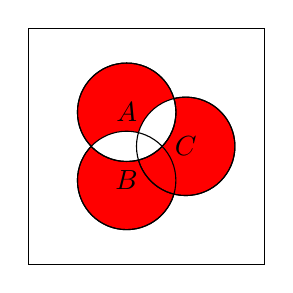
\begin{tikzpicture}[scale=0.5]
                  \draw (-3,-3) rectangle (3,3);

                  \begin{scope}[draw=transparent]
                      \draw[fill=red] (240:1) circle[radius=1.25];
                      \draw[fill=red] (360:1) circle[radius=1.25];
                      \draw[fill=red] (120:1) circle[radius=1.25];
                      \clip (240:1) circle[radius=1.25] (360:1) circle[radius=1.25];
                      \draw[fill=white] (120:1) circle[radius=1.25];
                  \end{scope}

                  \draw (120:1) node{$A$} circle[radius=1.25];
                  \draw (240:1) node{$B$} circle[radius=1.25];
                  \draw (360:1) node{$C$} circle[radius=1.25];
              \end{tikzpicture}
              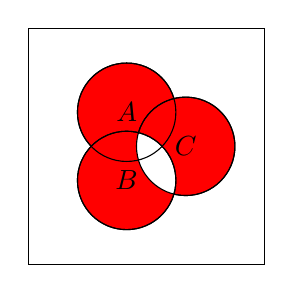
\begin{tikzpicture}[scale=0.5]
                  \draw (-3,-3) rectangle (3,3);
                  \begin{scope}[draw=transparent]
                      \draw[fill=red] (120:1) circle[radius=1.25];
                      \draw[fill=red] (360:1) circle[radius=1.25];
                      \draw[fill=red] (240:1) circle[radius=1.25];
                      \clip (360:1) circle[radius=1.25];
                      \clip (240:1) circle[radius=1.25];
                      \draw[fill=white] (240:1) circle[radius=1.25];
                  \end{scope}
                  %\draw[fill=red] (120:1) circle[radius=1.25];

                  \draw (120:1) node{$A$} circle[radius=1.25];
                  \draw (240:1) node{$B$} circle[radius=1.25];
                  \draw (360:1) node{$C$} circle[radius=1.25];
              \end{tikzpicture}
          \end{figure}

    \item Encontrar fórmulas que describan los siguientes diagramas de Venn, usando solo $\cup$, $\cap$ y $^c$
          \begin{enumerate}
              \item
                    \[ A - B = A \cap B^c \]
                    \[ (B \cap C) - A = (B \cap C) \cap A^c \]
                    \[ \boxed{(A \cap B^c) \cup (B \cap C \cap A^c)} \]
              \item
                    \[ A \triangle B = (A \cup C) - (A \cap C) = (A \cup C) \cap (A \cap C)^c \]
                    \[ (A \cup C) \cap (A \cap C)^c - B = \boxed{(A \cup C) \cap (A \cap C)^c \cap B^c} \]
              \item
                    \[ (A \cap B) \cup (B \cap C) \cup (C \cap A) \]
                    \[ (A \cap B) \cup (B \cap C) \cup (C \cap A) - (A \cap B \cap C) \]
                    \[ \boxed{(A \cap B) \cup (B \cap C) \cup (C \cap A) \cap (A \cap B \cap C)^c} \]
          \end{enumerate}

    \item 9lol

    \item Probar que $P(A) \subseteq P(B) \iff A \subseteq B$
          \begin{proof}
              Probar:
              \begin{itemize}
                  \item $A \subseteq B$
                  \item $\forall x \in A \implies x \in B$
              \end{itemize}
              Sea $x \in A$, $\{x\} \subseteq A$, por lo que $\{x\} \in P(A) \implies \{x\} \in P(B)$.
              Y por definicion de $P(B)$, $\{x\} \subseteq B$ por lo cual $x \in B$

              Probar:
              \begin{itemize}
                  \item $P(A) \subseteq P(B)$
                  \item $\forall c \in P(A) \implies c \in P(B)$
                  \item $\forall c \subseteq A \implies c \subseteq B$
              \end{itemize}

              Sea $c \in P(A)$, es decir $c \subseteq A$.
              Como $c \subseteq B$ y sabemos $A \subseteq B$ entonces $c \subseteq B$, o sea $c \in P(B)$
          \end{proof}

    \item Comparar las tablas de verdad de

          \begin{enumerate*}
              \item $p \implies q$
              \item $\neg p \implies \neg q$
              \item $\neg p \lor q$
              \item $\neg (p \land \neg q)$
          \end{enumerate*}
          \[
              \begin{array}{|c c|c|c c|c|c|c|c|}
                  p & q & p\implies q & \neg p & \neg q & \neg p \implies \neg q & \neg p \lor q & p \land \neg q & \neg (p \land \neg q) \\ \hline
                  V & V & V           & F      & F      & V                      & V             & F              & V                     \\
                  V & F & F           & F      & V      & V                      & F             & V              & F                     \\
                  F & V & V           & V      & F      & F                      & V             & F              & V                     \\
                  F & F & V           & V      & V      & V                      & V             & F              & V
              \end{array}
          \]

    \item \begin{enumerate}
              \item Decidir V ó F
                    \begin{enumerate}
                        \item $\forall n \in \N, n \geq 5$ \xmark $n = 4, n \not\geq 5 $
                        \item $\exists n \in \N, n \geq 5$ \cmark $n = 5, n \geq 5 $
                        \item $\forall n \in \N, n \geq 5 \lor n \leq 8$ \cmark $n \in \{3, 5, 8, 10\}$
                        \item $\exists n \in \N, n \geq 5 \land n \leq 8$ \cmark $n \in \{5, 6, 7, 8\}$
                        \item $\forall n \in \N, \exists m \in \N, m > n$ \cmark $n = 1, m = 2$. Para cualquier $n$, puedo tomar $m = n+1$ y va a ser mayor a $n$
                        \item $\exists n \in \N, \forall m \in \N, m > n$ \xmark Si tomamos $\neg p = \forall n \in \N, \exists m \in \N, m \leq n$, entonces podemos provar que $\neg p$ es verdadera:
                              \begin{proof}
                                  Si tomamos $n \in \N$, entonces podemos tomar $m = n$ y se cumple $m \leq n$
                              \end{proof}
                    \end{enumerate}
              \item Invertir las proposiciones anteriores
                    \begin{enumerate}
                        \item $\exists n \in \N, n < 5$
                        \item $\forall n \in \N, n < 5$
                        \item $\exists n \in \N, n < 5 \land n > 8$
                        \item $\forall n \in \N, n < 5 \lor n > 8$
                        \item $\exists n \in \N, \forall m \in \N, m \leq n$
                        \item $\forall n \in \N, \exists m \in \N, m \leq n$
                    \end{enumerate}
              \item Decidir si las siguientes proposiciones son iguales
                    \begin{enumerate}
                        \item $\exists x, \forall y, p(x, y)$ y $\forall y,\exists x, p(x, y)$ \xmark ver 12.a.5 y 12.a.6
                        \item $\forall x, p(x)$ y $\not\exists x, \neg p(x)$
                    \end{enumerate}

          \end{enumerate}

    \item Decidir V ó F y justificar
          \begin{enumerate}
              \item $(A \triangle B) - C = (A - C) \triangle (B - C)$ \cmark
                    \begin{proof}
                        \[ (A \triangle B) - C = (A - C) \triangle (B - C) \]
                        \bigskip
                        \begin{tabular}{|c c c|c|c|c|c|c|}
                            $A$ & $B$ & $C$ & $\smash{\overbrace{A \triangle B}^a}$ & $a - C$ & $\smash{\overbrace{A - C}^b}$ & $\smash{\overbrace{B - C}^c}$ & $b \triangle c$ \\ \hline
                            F   & F   & F   & F                                     & F       & F                             & F                             & F               \\
                            F   & F   & V   & F                                     & F       & F                             & F                             & F               \\
                            F   & V   & F   & V                                     & V       & F                             & V                             & V               \\
                            F   & V   & V   & V                                     & F       & F                             & F                             & F               \\
                            V   & F   & F   & V                                     & V       & V                             & F                             & V               \\
                            V   & F   & V   & V                                     & F       & F                             & F                             & F               \\
                            V   & V   & F   & F                                     & F       & V                             & V                             & F               \\
                            V   & V   & V   & F                                     & F       & F                             & F                             & F               \\
                        \end{tabular}
                    \end{proof}
              \item $A \triangle B \subseteq (A \triangle C) \cup (B \triangle C)$ \xmark
                    \begin{proof}
                        \[ A \triangle B \subseteq (A \triangle C) \cup (B \triangle C) \]
                        \bigskip
                        \begin{tabular}{|c c c|c|c|c|c|c|}
                            $A$ & $B$ & $C$ & $\smash{\overbrace{A \triangle B}^d}$ & $\smash{\overbrace{A \triangle C}^a}$ & $\smash{\overbrace{B \triangle C}^b}$ & $\smash{\overbrace{a \cup b}^c}$ & $d \subseteq c$ \\ \hline
                            F   & F   & F   & F                                     & F                                     & F                                     & F                                & V               \\
                            F   & F   & V   & F                                     & V                                     & V                                     & V                                & V               \\
                            F   & V   & F   & V                                     & F                                     & V                                     & V                                & V               \\
                            F   & V   & V   & V                                     & V                                     & F                                     & V                                & V               \\
                            V   & F   & F   & V                                     & V                                     & F                                     & V                                & V               \\
                            V   & F   & V   & V                                     & F                                     & V                                     & V                                & V               \\
                            V   & V   & F   & F                                     & V                                     & V                                     & V                                & V               \\
                            V   & V   & V   & F                                     & F                                     & F                                     & F                                & V               \\
                        \end{tabular}
                    \end{proof}
              \item $C \subseteq A \implies B \cap C \subseteq (A \triangle B)^c$ \cmark
                    \begin{proof}
                        \[ C \subseteq A \implies B \cap C \subseteq (A \triangle B)^c \]
                        es igual a
                        \[ (C \implies A) \implies ((B \land C) \implies \neg(A \veebar B)) \]
                        \bigskip
                        \begin{tabular}{|ccc|c|c|c|c|c|}
                            $A$ & $B$ & $C$ & $\smash{\overbrace{C \implies A}^a}$ & $\smash{\overbrace{B \land C}^b}$ & $\smash{\overbrace{\neg(A \veebar B)}^c}$ & $\smash{\overbrace{b \implies c}^d}$ & $a \implies d$ \\ \hline
                            F   & F   & F   & V                                    & F                                 & V                                         & V                                    & V              \\
                            F   & F   & V   & F                                    & F                                 & V                                         & V                                    & V              \\
                            F   & V   & F   & V                                    & F                                 & F                                         & V                                    & V              \\
                            F   & V   & V   & F                                    & V                                 & F                                         & F                                    & V              \\
                            V   & F   & F   & V                                    & F                                 & F                                         & V                                    & V              \\
                            V   & F   & V   & V                                    & F                                 & F                                         & V                                    & V              \\
                            V   & V   & F   & V                                    & F                                 & V                                         & V                                    & V              \\
                            V   & V   & V   & V                                    & V                                 & V                                         & V                                    & V              \\
                        \end{tabular}
                    \end{proof}
              \item $A \triangle B = \emptyset \iff A = B$
                    \begin{proof}
                        \[ A \triangle B = \emptyset \iff A = B \]
                        es igual a
                        \[ (A \veebar B = F) = (A = B) \]
                        \bigskip
                        \begin{tabular}{|c c|c|c|c|c|}
                            $A$ & $B$ & $\smash{\overbrace{A \veebar B}^a}$ & $\smash{\overbrace{a = F}^b}$ & $\smash{\overbrace{A = B}^c}$ & $b = c$ \\ \hline
                            F   & F   & F                                   & V                             & V                             & V       \\
                            F   & V   & V                                   & F                             & F                             & V       \\
                            V   & F   & V                                   & F                             & F                             & V       \\
                            V   & V   & F                                   & V                             & V                             & V       \\
                        \end{tabular}
                    \end{proof}

          \end{enumerate}

    \item 14lol

    \item \begin{enumerate}
              \item Diseñar para $A$, $B$ y $C$
                    \begin{enumerate}
                        \item $(A \cup B)' = A' \cup B'$
                        \item $-$
                        \item $-$
                        \item $-$
                        \item $-$
                        \item $A \triangle B = A-B \cap B -A = (A \cap B') \cup (B \cap A')$
                    \end{enumerate}
              \item
          \end{enumerate}

    \item Sean $A = \{1, 2, 3\}$ y $B = \{1, 3, 5, 7\}$. Hallar:
          \begin{enumerate}
              \item $A \x A =$
                    \[ \{ (1, 1), (1, 2), (1, 3), (2, 1), (2, 2), (2, 3), (3, 1), (3, 2), (3, 3) \} \]
              \item $A \x B = $
                    \[
                        \begin{Bmatrix}
                            (1, 1), (2, 1), (3, 1), \\
                            (1, 3), (2, 3), (3, 3), \\
                            (1, 5), (2, 5), (3, 5), \\
                            (1, 7), (2, 7), (3, 7)
                        \end{Bmatrix}
                    \]
              \item $(A \cap B) \x (A \cup B)$
                    \[ (A \cap B) = \{ 1, 3 \} \]
                    \[ (A \cup B) = \{ 1, 2, 3, 5, 7 \} \]
                    \[
                        \begin{Bmatrix}
                            (1,1),(3,1), \\
                            (1,2),(3,2)  \\
                            (1,3),(3,3)  \\
                            (1,5),(3,5)  \\
                            (1,7),(3,7)  \\
                        \end{Bmatrix}
                    \]
          \end{enumerate}

    \item 17lol

    \item Sean $A = \{1, 2, 3\}$ y $B = \{1, 3, 5, 7\}$. Verificar para cada caso si $R \subseteq A \x B$. En caso de ser verdadero, graficar
          \[
              A \x B = \begin{Bmatrix}
                  (1,1), & (2,1), & (3,1), \\
                  (1,3), & (2,3), & (3,3), \\
                  (1,5), & (2,5), & (3,5), \\
                  (1,7), & (2,7), & (3,7)  \\
              \end{Bmatrix}
          \]
          \begin{enumerate}
              \item $R = \{(1, 1), (1, 3), (1, 7), (3, 1), (3, 5)\}$ \cmark
              \item $R = \{(1, 1), (1, 3), (2, 7), (3, 2), (3, 5)\}$ \xmark
              \item $R = \{(1, 1), (1, 3), (2, 7), (3, 3), (3, 5)\}$ \cmark
              \item $R = \{(1, 1), (1, 3), (1, 7), (3, 1), (3, 3), (3, 7)\}$ \cmark
              \item $R = \{(1, 1), (1, 3), (3, 7)\}$ \cmark
              \item $R = \{(1, 3), (2, 3), (1, 7)\}$ \cmark
          \end{enumerate}
          \begin{enumerate*}
              \item 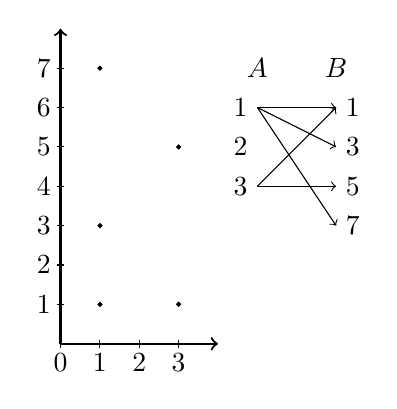
\begin{tikzpicture}[scale=0.5]
                  % Puntos
                  \begin{scope}[->,thick]
                      \draw (0,0) -- (0,8);
                      \draw (0,0) -- (4,0);
                  \end{scope}
                  \foreach \x in {0,1,2,3} {
                          \draw (\x,0) ++(0,0.1) -- ++(0,-0.2);
                          \draw (\x,0) node[anchor=north] {$\x$};
                      }
                  \foreach \y in {1,2,3,4,5,6,7} {
                          \draw (0,\y) ++(0.1,0) -- ++(-0.2,0);
                          \draw (0,\y) node[anchor=east] {$\y$};
                      }
                  \begin{scope}[radius=0.05]
                      \draw[fill=black] (1,1) circle;
                      \draw[fill=black] (1,3) circle;
                      \draw[fill=black] (1,7) circle;
                      \draw[fill=black] (3,1) circle;
                      \draw[fill=black] (3,5) circle;
                  \end{scope}

                  % Venn
                  \coordinate (A1) at (5,6);
                  \coordinate (A2) at (5,5);
                  \coordinate (A3) at (5,4);

                  \coordinate (B1) at (7,6);
                  \coordinate (B3) at (7,5);
                  \coordinate (B5) at (7,4);
                  \coordinate (B7) at (7,3);

                  \draw (5,7) node{$A$};
                  \draw (7,7) node{$B$};

                  \begin{scope}[anchor=east]
                      \draw (A1) node{$1$};
                      \draw (A2) node{$2$};
                      \draw (A3) node{$3$};
                  \end{scope}
                  \begin{scope}[anchor=west]
                      \draw (B1) node {$1$};
                      \draw (B3) node {$3$};
                      \draw (B5) node {$5$};
                      \draw (B7) node {$7$};
                  \end{scope}
                  \begin{scope}[->]
                      \draw (A1) -- (B1);
                      \draw (A1) -- (B3);
                      \draw (A1) -- (B7);
                      \draw (A3) -- (B1);
                      \draw (A3) -- (B5);
                  \end{scope}
              \end{tikzpicture}

              \item \xmark \\

              \item 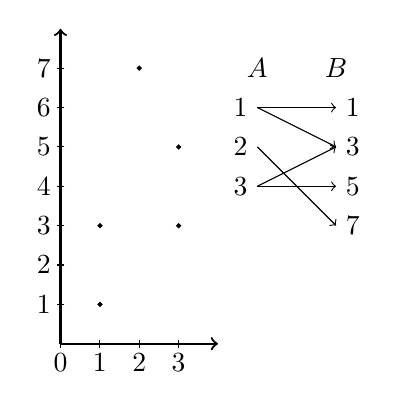
\begin{tikzpicture}[scale=0.5]
                  \begin{scope}[->,thick]
                      \draw (0,0) -- (0,8);
                      \draw (0,0) -- (4,0);
                  \end{scope}
                  \foreach \x in {0,1,2,3} {
                          \draw (\x,0) ++(0,0.1) -- ++(0,-0.2);
                          \draw (\x,0) node[anchor=north] {$\x$};
                      }
                  \foreach \y in {1,2,3,4,5,6,7} {
                          \draw (0,\y) ++(0.1,0) -- ++(-0.2,0);
                          \draw (0,\y) node[anchor=east] {$\y$};
                      }
                  \begin{scope}[radius=0.05]
                      \draw[fill=black] (1,1) circle;
                      \draw[fill=black] (1,3) circle;
                      \draw[fill=black] (2,7) circle;
                      \draw[fill=black] (3,3) circle;
                      \draw[fill=black] (3,5) circle;
                  \end{scope}

                  % Venn
                  \coordinate (A1) at (5,6);
                  \coordinate (A2) at (5,5);
                  \coordinate (A3) at (5,4);

                  \coordinate (B1) at (7,6);
                  \coordinate (B3) at (7,5);
                  \coordinate (B5) at (7,4);
                  \coordinate (B7) at (7,3);

                  \draw (5,7) node{$A$};
                  \draw (7,7) node{$B$};

                  \begin{scope}[anchor=east]
                      \draw (A1) node{$1$};
                      \draw (A2) node{$2$};
                      \draw (A3) node{$3$};
                  \end{scope}
                  \begin{scope}[anchor=west]
                      \draw (B1) node {$1$};
                      \draw (B3) node {$3$};
                      \draw (B5) node {$5$};
                      \draw (B7) node {$7$};
                  \end{scope}
                  \begin{scope}[->]
                      \draw (A1) -- (B1);
                      \draw (A1) -- (B3);
                      \draw (A2) -- (B7);
                      \draw (A3) -- (B3);
                      \draw (A3) -- (B5);
                  \end{scope}
              \end{tikzpicture}

              \item 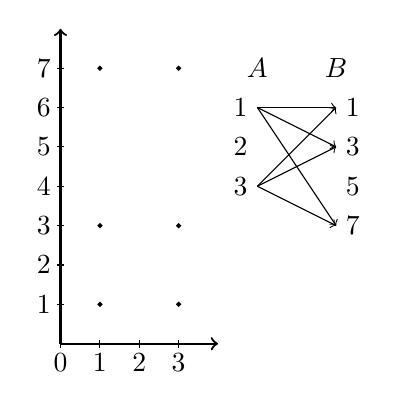
\begin{tikzpicture}[scale=0.5]
                  \begin{scope}[->,thick]
                      \draw (0,0) -- (0,8);
                      \draw (0,0) -- (4,0);
                  \end{scope}
                  \foreach \x in {0,1,2,3} {
                          \draw (\x,0) ++(0,0.1) -- ++(0,-0.2);
                          \draw (\x,0) node[anchor=north] {$\x$};
                      }
                  \foreach \y in {1,2,3,4,5,6,7} {
                          \draw (0,\y) ++(0.1,0) -- ++(-0.2,0);
                          \draw (0,\y) node[anchor=east] {$\y$};
                      }
                  \begin{scope}[radius=0.05]
                      \draw[fill=black] (1,1) circle;
                      \draw[fill=black] (1,3) circle;
                      \draw[fill=black] (1,7) circle;
                      \draw[fill=black] (3,1) circle;
                      \draw[fill=black] (3,3) circle;
                      \draw[fill=black] (3,7) circle;
                  \end{scope}

                  % Venn
                  \coordinate (A1) at (5,6);
                  \coordinate (A2) at (5,5);
                  \coordinate (A3) at (5,4);

                  \coordinate (B1) at (7,6);
                  \coordinate (B3) at (7,5);
                  \coordinate (B5) at (7,4);
                  \coordinate (B7) at (7,3);

                  \draw (5,7) node{$A$};
                  \draw (7,7) node{$B$};

                  \begin{scope}[anchor=east]
                      \draw (A1) node{$1$};
                      \draw (A2) node{$2$};
                      \draw (A3) node{$3$};
                  \end{scope}
                  \begin{scope}[anchor=west]
                      \draw (B1) node {$1$};
                      \draw (B3) node {$3$};
                      \draw (B5) node {$5$};
                      \draw (B7) node {$7$};
                  \end{scope}
                  \begin{scope}[->]
                      \draw (A1) -- (B1);
                      \draw (A1) -- (B3);
                      \draw (A1) -- (B7);
                      \draw (A3) -- (B1);
                      \draw (A3) -- (B3);
                      \draw (A3) -- (B7);
                  \end{scope}
              \end{tikzpicture} \\

              \item 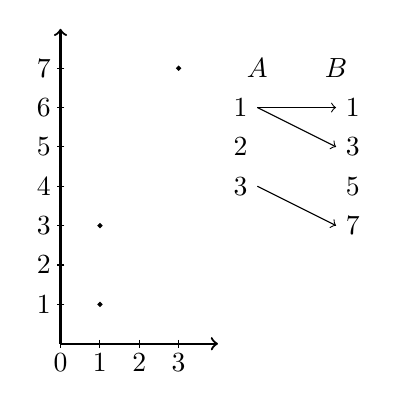
\begin{tikzpicture}[scale=0.5]
                  \begin{scope}[->,thick]
                      \draw (0,0) -- (0,8);
                      \draw (0,0) -- (4,0);
                  \end{scope}
                  \foreach \x in {0,1,2,3} {
                          \draw (\x,0) ++(0,0.1) -- ++(0,-0.2);
                          \draw (\x,0) node[anchor=north] {$\x$};
                      }
                  \foreach \y in {1,2,3,4,5,6,7} {
                          \draw (0,\y) ++(0.1,0) -- ++(-0.2,0);
                          \draw (0,\y) node[anchor=east] {$\y$};
                      }
                  \begin{scope}[radius=0.05]
                      \draw[fill=black] (1,1) circle;
                      \draw[fill=black] (1,3) circle;
                      \draw[fill=black] (3,7) circle;
                  \end{scope}

                  % Venn
                  \coordinate (A1) at (5,6);
                  \coordinate (A2) at (5,5);
                  \coordinate (A3) at (5,4);

                  \coordinate (B1) at (7,6);
                  \coordinate (B3) at (7,5);
                  \coordinate (B5) at (7,4);
                  \coordinate (B7) at (7,3);

                  \draw (5,7) node{$A$};
                  \draw (7,7) node{$B$};

                  \begin{scope}[anchor=east]
                      \draw (A1) node{$1$};
                      \draw (A2) node{$2$};
                      \draw (A3) node{$3$};
                  \end{scope}
                  \begin{scope}[anchor=west]
                      \draw (B1) node {$1$};
                      \draw (B3) node {$3$};
                      \draw (B5) node {$5$};
                      \draw (B7) node {$7$};
                  \end{scope}
                  \begin{scope}[->]
                      \draw (A1) -- (B1);
                      \draw (A1) -- (B3);
                      \draw (A3) -- (B7);
                  \end{scope}
              \end{tikzpicture}

              \item 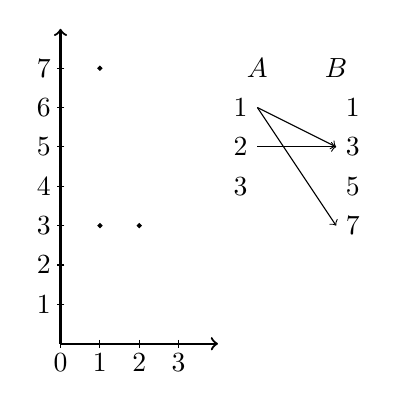
\begin{tikzpicture}[scale=0.5]
                  \begin{scope}[->,thick]
                      \draw (0,0) -- (0,8);
                      \draw (0,0) -- (4,0);
                  \end{scope}
                  \foreach \x in {0,1,2,3} {
                          \draw (\x,0) ++(0,0.1) -- ++(0,-0.2);
                          \draw (\x,0) node[anchor=north] {$\x$};
                      }
                  \foreach \y in {1,2,3,4,5,6,7} {
                          \draw (0,\y) ++(0.1,0) -- ++(-0.2,0);
                          \draw (0,\y) node[anchor=east] {$\y$};
                      }
                  \begin{scope}[radius=0.05]
                      \draw[fill=black] (1,3) circle;
                      \draw[fill=black] (2,3) circle;
                      \draw[fill=black] (1,7) circle;
                  \end{scope}

                  % Venn
                  \coordinate (A1) at (5,6);
                  \coordinate (A2) at (5,5);
                  \coordinate (A3) at (5,4);

                  \coordinate (B1) at (7,6);
                  \coordinate (B3) at (7,5);
                  \coordinate (B5) at (7,4);
                  \coordinate (B7) at (7,3);

                  \draw (5,7) node{$A$};
                  \draw (7,7) node{$B$};

                  \begin{scope}[anchor=east]
                      \draw (A1) node{$1$};
                      \draw (A2) node{$2$};
                      \draw (A3) node{$3$};
                  \end{scope}
                  \begin{scope}[anchor=west]
                      \draw (B1) node {$1$};
                      \draw (B3) node {$3$};
                      \draw (B5) node {$5$};
                      \draw (B7) node {$7$};
                  \end{scope}
                  \begin{scope}[->]
                      \draw (A1) -- (B3);
                      \draw (A2) -- (B3);
                      \draw (A1) -- (B7);
                  \end{scope}
              \end{tikzpicture}

          \end{enumerate*}

    \item Sean $A = \{1, 2, 3\}$ y $B = \{1, 3, 5, 7\}$. Describir por extensión cada caso de $R$
          \[
              A \x B = \begin{Bmatrix}
                  (1,1), & (2,1), & (3,1), \\
                  (1,3), & (2,3), & (3,3), \\
                  (1,5), & (2,5), & (3,5), \\
                  (1,7), & (2,7), & (3,7)  \\
              \end{Bmatrix}
          \]
          \begin{enumerate}
              \item $(a, b) \in R \iff a \leq b$
                    \[
                        \begin{Bmatrix}
                            (1,1), &        &        \\
                            (1,3), & (2,3), & (3,3), \\
                            (1,5), & (2,5), & (3,5), \\
                            (1,7), & (2,7), & (3,7)  \\
                        \end{Bmatrix}
                    \]
              \item $(a, b) \in R \iff a > b$
                    \[ \{ (2, 1), (3, 1) \} \]
              \item $(a, b) \in R \iff a \cdot b$ es par
                    \[ \{ (2, 1), (2, 3), (2, 5), (2, 7) \} \]
              \item $(a, b) \in R \iff a + b > 6$
                    \[ \{ (2, 5), (3, 5), (1, 7), (2, 7), (3, 7) \} \]
          \end{enumerate}

    \item Sea $A = \{a, b, c, d, e, f, g, h\}$. Para cada caso describir por extensión y determinar si es: Reflexiva, anti/simétrica o transitiva
          \begin{enumerate}
              \item $\{ (a, b), (b, a), (f, f), (c, c), (c, d), (c, h), (e, c), (h, g) \}$
                    \begin{itemize}
                        \item Reflexiva \xmark: $g \notrel g$
                        \item Simétrica \xmark: $h \rel g$ pero $h \notrel g$
                        \item Antisimétrica \cmark
                        \item Transitiva \xmark: $c \rel h$, $h \rel g$ pero $c \notrel g$
                    \end{itemize}
              \item $\{ (a, a), (b, b), (c, c), (d, d), (e, e), (f, f), (g, g), (h, h), \\ (a, b), (b, a), (d, c), (c, d), (c, e), (c, h), (h, g) \}$
                    \begin{itemize}
                        \item Reflexiva \cmark
                        \item Simétrica \xmark: $c \rel h$ pero $h \notrel c$
                        \item Antisimétrica \xmark: $c \rel d$ y $d \rel c$
                        \item Transitiva \xmark: $c \rel h$, $h \rel g$ pero $c \notrel g$
                    \end{itemize}
              \item $\{ (a, a), (b, b), (c, c), (f, f), (a, b), (b, a), (c, e), (c, h), (c, h), (h, g) \}$
                    \begin{itemize}
                        \item Reflexiva \xmark: $d \notrel d$
                        \item Simétrica \xmark: $c \rel e$ pero $e \notrel c$
                        \item Antisimétrica \xmark: $a \rel b$ y $b \rel a$
                        \item Transitiva \cmark: $c \rel h$, $h \rel g$ y $c \rel g$
                    \end{itemize}
              \item $\{ (a, a), (b, b), (c, c), (d, d), (e, e), (f, f), (g, g), (h, h), \\ (a, b), (b, a), (e, h), (h, e), (e, g), (g, e), (h, g), (h, g) \}$
                    \begin{itemize}
                        \item Reflexiva \cmark
                        \item Simétrica \cmark: $a$ con $b$; $g$, $h$ y $e$
                        \item Antisimétrica \xmark: $a \rel b$ y $b \rel a$
                        \item Transitiva \cmark: $g$, $h$ y $e$
                    \end{itemize}
          \end{enumerate}
    \item Graficar $R = \{ (1, 1), (1, 3), (3, 1), (3, 3), (6, 4), (4, 6), (4, 4), (6, 6) \}$

          \begin{tikzpicture}
              \coordinate (1) at (0,0);
              \coordinate (3) at (2,0);
              \coordinate (4) at (0,2);
              \coordinate (6) at (2,2);

              \draw (1) node[above]{$1$};
              \draw (3) node[above]{$3$};
              \draw (4) node[below]{$4$};
              \draw (6) node[below]{$6$};

              \begin{scope}[->, thick]
                  \path (1) edge [loop below] node {} ();
                  \path (3) edge [loop below] node {} ();
                  \path (4) edge [loop above] node {} ();
                  \path (6) edge [loop above] node {} ();
                  \draw[<->] ($(1)!.9!(3)$) -- ($(3)!.9!(1)$);
                  \draw[<->] ($(6)!.9!(4)$) -- ($(4)!.9!(6)$);
              \end{scope}
          \end{tikzpicture}

    \item Sea $A = \{a, b, c, d, e, f\}$ y sea $R$ el grafico:
          Hallar los pares a añadir para que $R$ sea
          \begin{enumerate}
              \item Reflexiva: $\{(b, b), (c, c), (d, d), (f, f)\}$
              \item Simétrica: $(c, b)$
              \item Transitiva: $\{(c, f), (b, f)\}$
              \item Reflexiva y simétrica: $\{(b, b), (c, c), (d, d), (f, f), (c, b)\}$
              \item Simétrica y transitiva: $\{(c, b), (b, f), (c, f)\}$
              \item Equivalencia % ???
          \end{enumerate}
    \item Determinar si $R$ es reflexica, anti/simétrica, transitiva, de equivalencia o de orden
          \begin{enumerate}
              \item $A = \{1, 2, 3, 4, 5\}$, $R = \{(1, 1), (2, 2), (3, 3), (4, 4), (5, 5)\}$: Reflexiva
              \item $A = \{1, 2, 3, 4, 5, 6\}$, $R = \{(1, 1), (2, 2), (3, 3), (4, 4), (5, 5), (6, 6)\}$: Reflexiva
              \item $A = \{1, 2, 3, 4, 5\}$, $R = \{(1, 1),(2, 2),(3, 3),(4, 4),(5, 5),(1, 2),(1, 3),(2, 5),(1, 5)\}$
              \item $A = \N$, $R = \{(a, b) \in \N \x \N / a + b \text{ es par}\}$
                    \[ R = \{(a, b) \in \N \x \N / a + b = 2k, k \in \Z \} \]
              \item $A = Z$, $R = \{(a, b) \in \Z \x \Z / |a| \leq |b|\}$
              \item $A = N$, $R$ definida por $a \rel b \iff b$ es múltiplo de $a$
              \item $A = P(R)$, $R$ definida por $X \rel Y \iff X \cap \{1, 2, 3\} \subseteq Y \cap \{1, 2, 3\}$
          \end{enumerate}
    \item 24lol
    \item En $R$ de equivalencia en $A$, hallar clases $\overline{a}$ de $a$, $\overline{b}$ de $b$, $\overline{c}$ de $c$, $\overline{d}$ de $d$ y la partición asociada a $R$
          \begin{align*}
              R = \{ & (a, a), (b, b), (c, c), (d, d), (e, e), (f, f),                  \\
                     & (a, b), (b, a), (a, f), (f, a), (b, f), (f, b), (c, e), (e, c)\}
          \end{align*}
          \begin{figure*}[h]
              \centering
              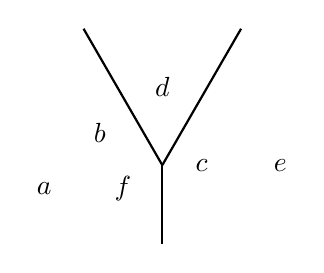
\begin{tikzpicture}
                  \node (c) at (0.5,0) {$c$};
                  \node (e) [right of=c] {$e$};
                  \node (d) at (90:1) {$d$};
                  \node (a) at (-1.5,-0.3) {$a$};
                  \node (b) [above right of=a] {$b$};
                  \node (f) [right of=a] {$f$};
                  \begin{scope}[thick]
                      \draw (60:2) -- (0,0);
                      \draw (120:2) -- (0,0);
                      \draw (270:1) -- (0,0);
                  \end{scope}
              \end{tikzpicture}
          \end{figure*}

          \begin{itemize}
              \item $\overline{a} = \overline{b} = \overline{f} =\{a, b, f\}$
              \item $\overline{d} = \{d\}$
              \item $\overline{c} = \overline{e} = \{c, e\}$
              \item Partición $= \{\{a, b, c\}, \{c, e\}, \{d\}\}$
          \end{itemize}
    \item Sea $A = \{1, 2, ..., 9, 10\}$ hallar y grafica la $R$ de equivalencia de la partición $\{\{1, 3\}, \{2, 6, 7\}, \{4, 8, 9, 10\}, \{5\}\}$.

          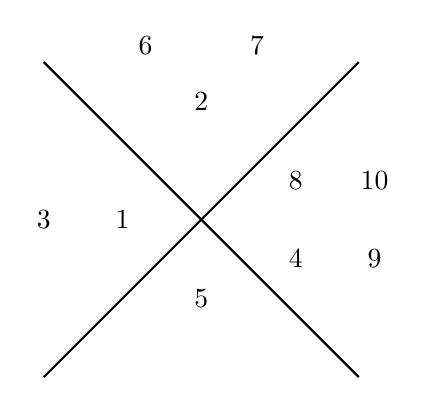
\begin{tikzpicture}
              \node (1) at (-1,0) {$1$};
              \node (3) [left of=1] {$3$};

              \node (2) at (0,1.5) {$2$};
              \node (6) [above left of=2] {$6$};
              \node (7) [above right of=2] {$7$};

              \node (4) at (1.2,-0.5) {$4$};
              \node (8) [above of=4] {$8$};
              \node (9) [right of=4] {$9$};
              \node (10) [above of=9] {$10$};

              \node (5) at (0,-1) {$5$};

              \begin{scope}[thick]
                  \draw (-2,2) -- (2,-2);
                  \draw (-2,-2) -- (2,2);
              \end{scope}

          \end{tikzpicture}

    \item 27lol
    \item 28lol
    \item 29lol

\end{enumerate}

\end{document}